% Five horizontal lines, a sample of the meagre union over rational heights. The complement is residual.
\begin{tikzpicture}[x=1.05cm,y=1.05cm,font=\footnotesize]
  \fill[MidnightBlue!14] (0,0) rectangle (6.4,4.2);
  \draw[MidnightBlue] (0,0) rectangle (6.4,4.2);
  \draw[BurntOrange,line width=0.9pt] (0,0.45)--(6.4,0.45);
  \draw[BurntOrange,line width=0.9pt] (0,1.25)--(6.4,1.25);
  \draw[BurntOrange,line width=0.9pt] (0,2.10)--(6.4,2.10);
  \draw[BurntOrange,line width=0.9pt] (0,2.95)--(6.4,2.95);
  \draw[BurntOrange,line width=0.9pt] (0,3.70)--(6.4,3.70);
  \node[text=BurntOrange,anchor=east] at (-0.06,0.45) {$0$};
  \node[text=BurntOrange,anchor=east] at (-0.06,1.25) {$\tfrac12$};
  \node[text=BurntOrange,anchor=east] at (-0.06,2.10) {$1$};
  \node[text=BurntOrange,anchor=east] at (-0.06,2.95) {$\tfrac32$};
  \node[text=BurntOrange,anchor=east] at (-0.06,3.70) {$2$};
  % Disc centred on the line y=1: it is not contained in the line.
  \draw[MidnightBlue,line width=0.8pt] (1.7,2.10) circle (0.48);
  \node[text=MidnightBlue,anchor=west] at (2.28,2.10) {meets the line};
  % Open piece of the complement, between y=1 and y=3/2.
  \fill[MidnightBlue!45] (4.7,2.52) circle (0.26);
  \draw[MidnightBlue,line width=0.7pt] (4.7,2.52) circle (0.26);
  \node[text=MidnightBlue,anchor=west] at (5.08,2.52) {in the complement};
\end{tikzpicture}
